\chapter{The Large Hadron Collider \label{chap:LHC}}

The Large Hadron Collider (LHC) is the world's largest particle accelerator and collider, able to
reach unprecedented particle energies. It is located at CERN, the European Organization for Nuclear
Research on the Swiss-French border near Geneva, in the 27 kilometre long tunnel that previously
housed the Large Electron Positron (LEP) collider. The LHC consists of a sequence of superconducting
magnets that guide two proton beams in opposite directions around the LHC ring, which is composed
of 8 straight and 8 curved sections. 
The beams are accelerated at each turn around the ring, and are made to collide in four interaction
points.
If operating at design conditions, the LHC would provide 600 million $\Pp\Pp$
collisions per second, at a centre-of-mass energy of 14\TeV and a luminosity of
$\text{10}^\text{34}\percms$. 
In the next sections I will highlight some of the main features of the LHC. A more comprehensive
discussion
can be found in Refs.~\cite{Evans:2008zzb,Bruning:2007zzc,Lefevre:1165534,LHC_website}. 

\section{A proton machine \label{sec:LHC_proton_machine}}

Both LHC beams contain protons, unlike the previous large accelerators LEP and Tevatron which
collided electrons on positrons, and protons on anti-protons, respectively. 
The decision to use solely protons was driven by the purpose of the LHC: to be a discovery machine.
The LHC was built to test the Standard Model at never seen energies, provide enough data to
probe very rare processes, and hopefully discover new particles. So far the LHC has lived up to
expectation. Per beam energies of up to 4\TeV were reached, providing access to a completely new
energy domain. In 2012 the discovery of the long-sought-after Higgs boson was announced, followed in
2013 by a Nobel prize for Fran\c{c}ois Englert and Peter Higgs, the theorists that first proposed
the existence of this particle. 

The advantage protons have over electrons and positrons is their 2000 times larger mass, resulting
in a much reduced energy loss due to synchrotron radiation. This allows the LHC beam to reach
energies that would be impossible at LEP.
The drawback is the proton's complex structure. Electrons are fundamental particles, which
means that the centre-of-mass energy of the collision is precisely known. This is not the case for
protons. In a $\Pp\Pp$ collision we know the energy of the protons, but not of the individual quarks
and gluons inside the proton that participate in the hard interaction. Consequently, each collision
has a different centre-of-mass energy, making it hard to perform precision measurements. The
compositeness
of the protons also leads to messier collisions, as the proton remnants can also interact and
obscure the interesting hard collision event. 

The LHC was built as a $\Pp\Pp$ machine rather than a $\Pp\Pap$ machine because anti-protons are
hard to produce and unstable, thus limiting the maximal luminosity that can be achieved. Of course,
there is also a downside here. A proton and anti-proton beam can be circulated in opposite
directions using the same magnetic field, and thus beam pipe. However, to steer two proton beams in
opposite direction, we need to apply an opposite magnetic field, meaning that two separate beam
pipes are needed. 


\section{Superconducting magnets}

In order to reach the design centre-of-mass energy of 14\TeV, conventional magnets do not
suffice. Therefore, superconducting magnets were used instead. They can provide the very high
magnetic fields, up to 8.4\unit{T} for the LHC magnets, needed to bend the highly energetic
particles around the ring, at reasonable power consumption. The magnet coils are built from
niobium-titanium
cable, that when cooled to 1.9\unit{K} attains a superconducting state, allowing electricity to flow
without resistance. The cryostat at the LHC is of unseen proportion, stretching along the
27\unit{km} long ring, and containing 120 tonnes of helium.

The need for two separate beam pipes caused some complication for the LHC design. The LEP tunnel is
quite narrow, too narrow, in fact, to hold two completely separate proton rings. A solution was
found in the so-called twin-bore, or two-in-one, magnet design. This design accommodates the
windings for both beam channels in a common cold mass and cryostat, with the magnetic flux
circulating in the opposite sense through the two channels. 
It also makes the magnet structure more complicated, as the separation between the two channels is
small enough that they are coupled both magnetically and mechanically. An illustration of the
twin-bore design is shown in Fig.~\ref{fig:lhc_twin_bore}. 

Guiding beams around the LHC ring requires thousands of magnets of different varieties and sizes.
Beams are bent by a total of 1232 dipole magnets, 15 metres in length, and are focussed by 392
quadrupole magnets, each 5–7 metres long. Different kinds of multipole magnets are used to correct
small imperfections in the magnetic field at the ends of the dipoles. So-called insertion magnets
are used to squeeze the beam from 0.2 millimetres down to 16 micrometres across, just before it
reaches one of the detectors in the interaction points. 

\begin{figure}[t]
  \centering
  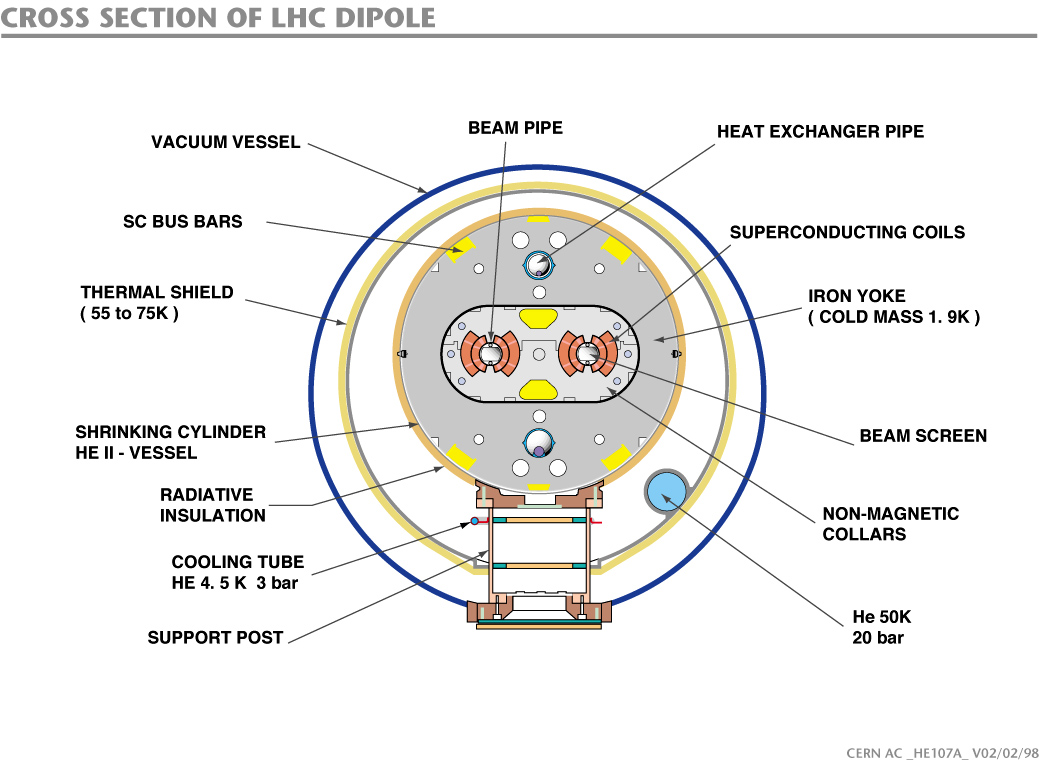
\includegraphics[width=\textwidth,clip=true,trim=0 2cm 0 2cm]
  {figures/lhc/lhc_dipole_cross_section_cds841539.jpg} 
  \caption{Cross section of an LHC dipole magnet, illustrating the twin-bore magnet
design~\cite{cds:841539}. The two beam pipes surrounded by the dipole magnets are clearly
visible. They are encased in a single cold volume and vacuum vessel. 
  \label{fig:lhc_twin_bore}}
\end{figure}


\section{Accelerating cavities}

The necessary accelerating power to raise the beam energy from the injection energy of 450\GeV to
the collision energy of several \TeV is provided by eight radiofrequency (RF) cavities per beam. 

RF cavities are metal chambers, often structured like beads on a string, where the beads are the
cavities and the string is the beam pipe of the accelerator.
An electromagnetic (EM) field is supplied to the cavities by an RF power generator. The specific
shape and size of the cavities are such that the EM waves become resonant, and build up inside the
cavity. 
Charged particles passing through the cavity feel the force and direction of the resulting
electromagnetic field, and are pulled along with the field. 
As the field in the LHC RF cavities oscillates at 400\unit{MHz}, the arrival of the protons needs to
be timed precisely in order for them to be accelerated, and not decelerated, see 
Fig.~\ref{fig:RF_explanation}. 
Once the particles have circled the LHC ring a sufficient number of times, passing through
the RF cavities on each turn, they attain the desired energy. At this point the main purpose of the
RF cavities is to keep the protons inside their \textit{bunches}. 

\begin{figure}[htpb]
  \centering
  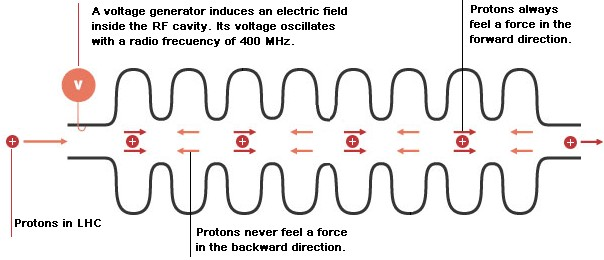
\includegraphics[width=0.8\textwidth]{figures/lhc/RF_explanation}
  \caption{Interaction between a proton and the oscillating electromagnetic field inside a
radiofrequency cavity. Figure taken from Ref.~\cite{RF_explanation}.
  \label{fig:RF_explanation}}
\end{figure}

The protons in the LHC beams do not form a continuous flow, but are grouped in packets, the bunches,
with empty space in between. Up to 2808 bunches can circle the LHC at any
given time. An ideally timed proton, with exactly the right energy, will see zero
accelerating voltage from the RF cavities when the LHC is at full energy. Protons with slightly
different energies arriving earlier or later will be accelerated or decelerated so that they stay
close to the energy of the ideal particle. In this way, the beam bunches stay intact. 

The LHC utilizes superconducting RF cavities made of niobium sputtered on copper, which are
cooled to 4.5\unit{K}. The RF power, up to 2\unit{MV} per cavity, is delivered by klystrons and
passed to the cavities via waveguides. Protons can thus gain up to 16\MeV per turn around the ring.
The RF cavities are grouped by fours in cryomodules, which are installed in a straight section of
the LHC tunnel. 

\section{LHC accelerator complex and experiments}

Up to now I have mainly covered what happens to a proton once it enters the LHC ring. In this
section I will briefly discuss the many steps the protons go through prior to entering the LHC,
and how they leave it again. 

It all starts with a bottle of hydrogen. Protons are obtained by applying an electromagnetic field
to strip off the electrons from the hydrogen atoms. The protons pass through a linear accelerator,
the Linac 2, where they obtain an energy of 50\MeV, and are then injected into the Proton
Synchrotron (PS) Booster. The booster accelerates the protons to 1.4\GeV at which point the beam is
fed to the PS where it attains an energy of 25\GeV. From the PS the beam is sent to the Super Proton
Synchrotron (SPS) where the protons reach an energy of 450\GeV. 
The beams are then finally transferred to the LHC, both in a clockwise and an anticlockwise
direction, where they are accelerated to their final energy. This entire process is illustrated in
Fig.~\ref{fig:lhc_complex}. 

In addition to accelerating protons, the accelerator complex can also accelerate lead ions, which
are produced from a highly purified lead sample, heated to a temperature of about500$\de$C. An
electric current is used to ionize the lead vapour.
The lead ions pass through Linac 3, and are then accumulated and accelerated to 72\MeV per nucleon
in the Low Energy Ion Ring (LEIR). 
From the LEIR the ions are transferred to the PS, from where they follow the same path as the
protons, reaching a final energy of 2.76\TeV per nucleon in the LHC. 

\begin{figure}[t]
  \centering
  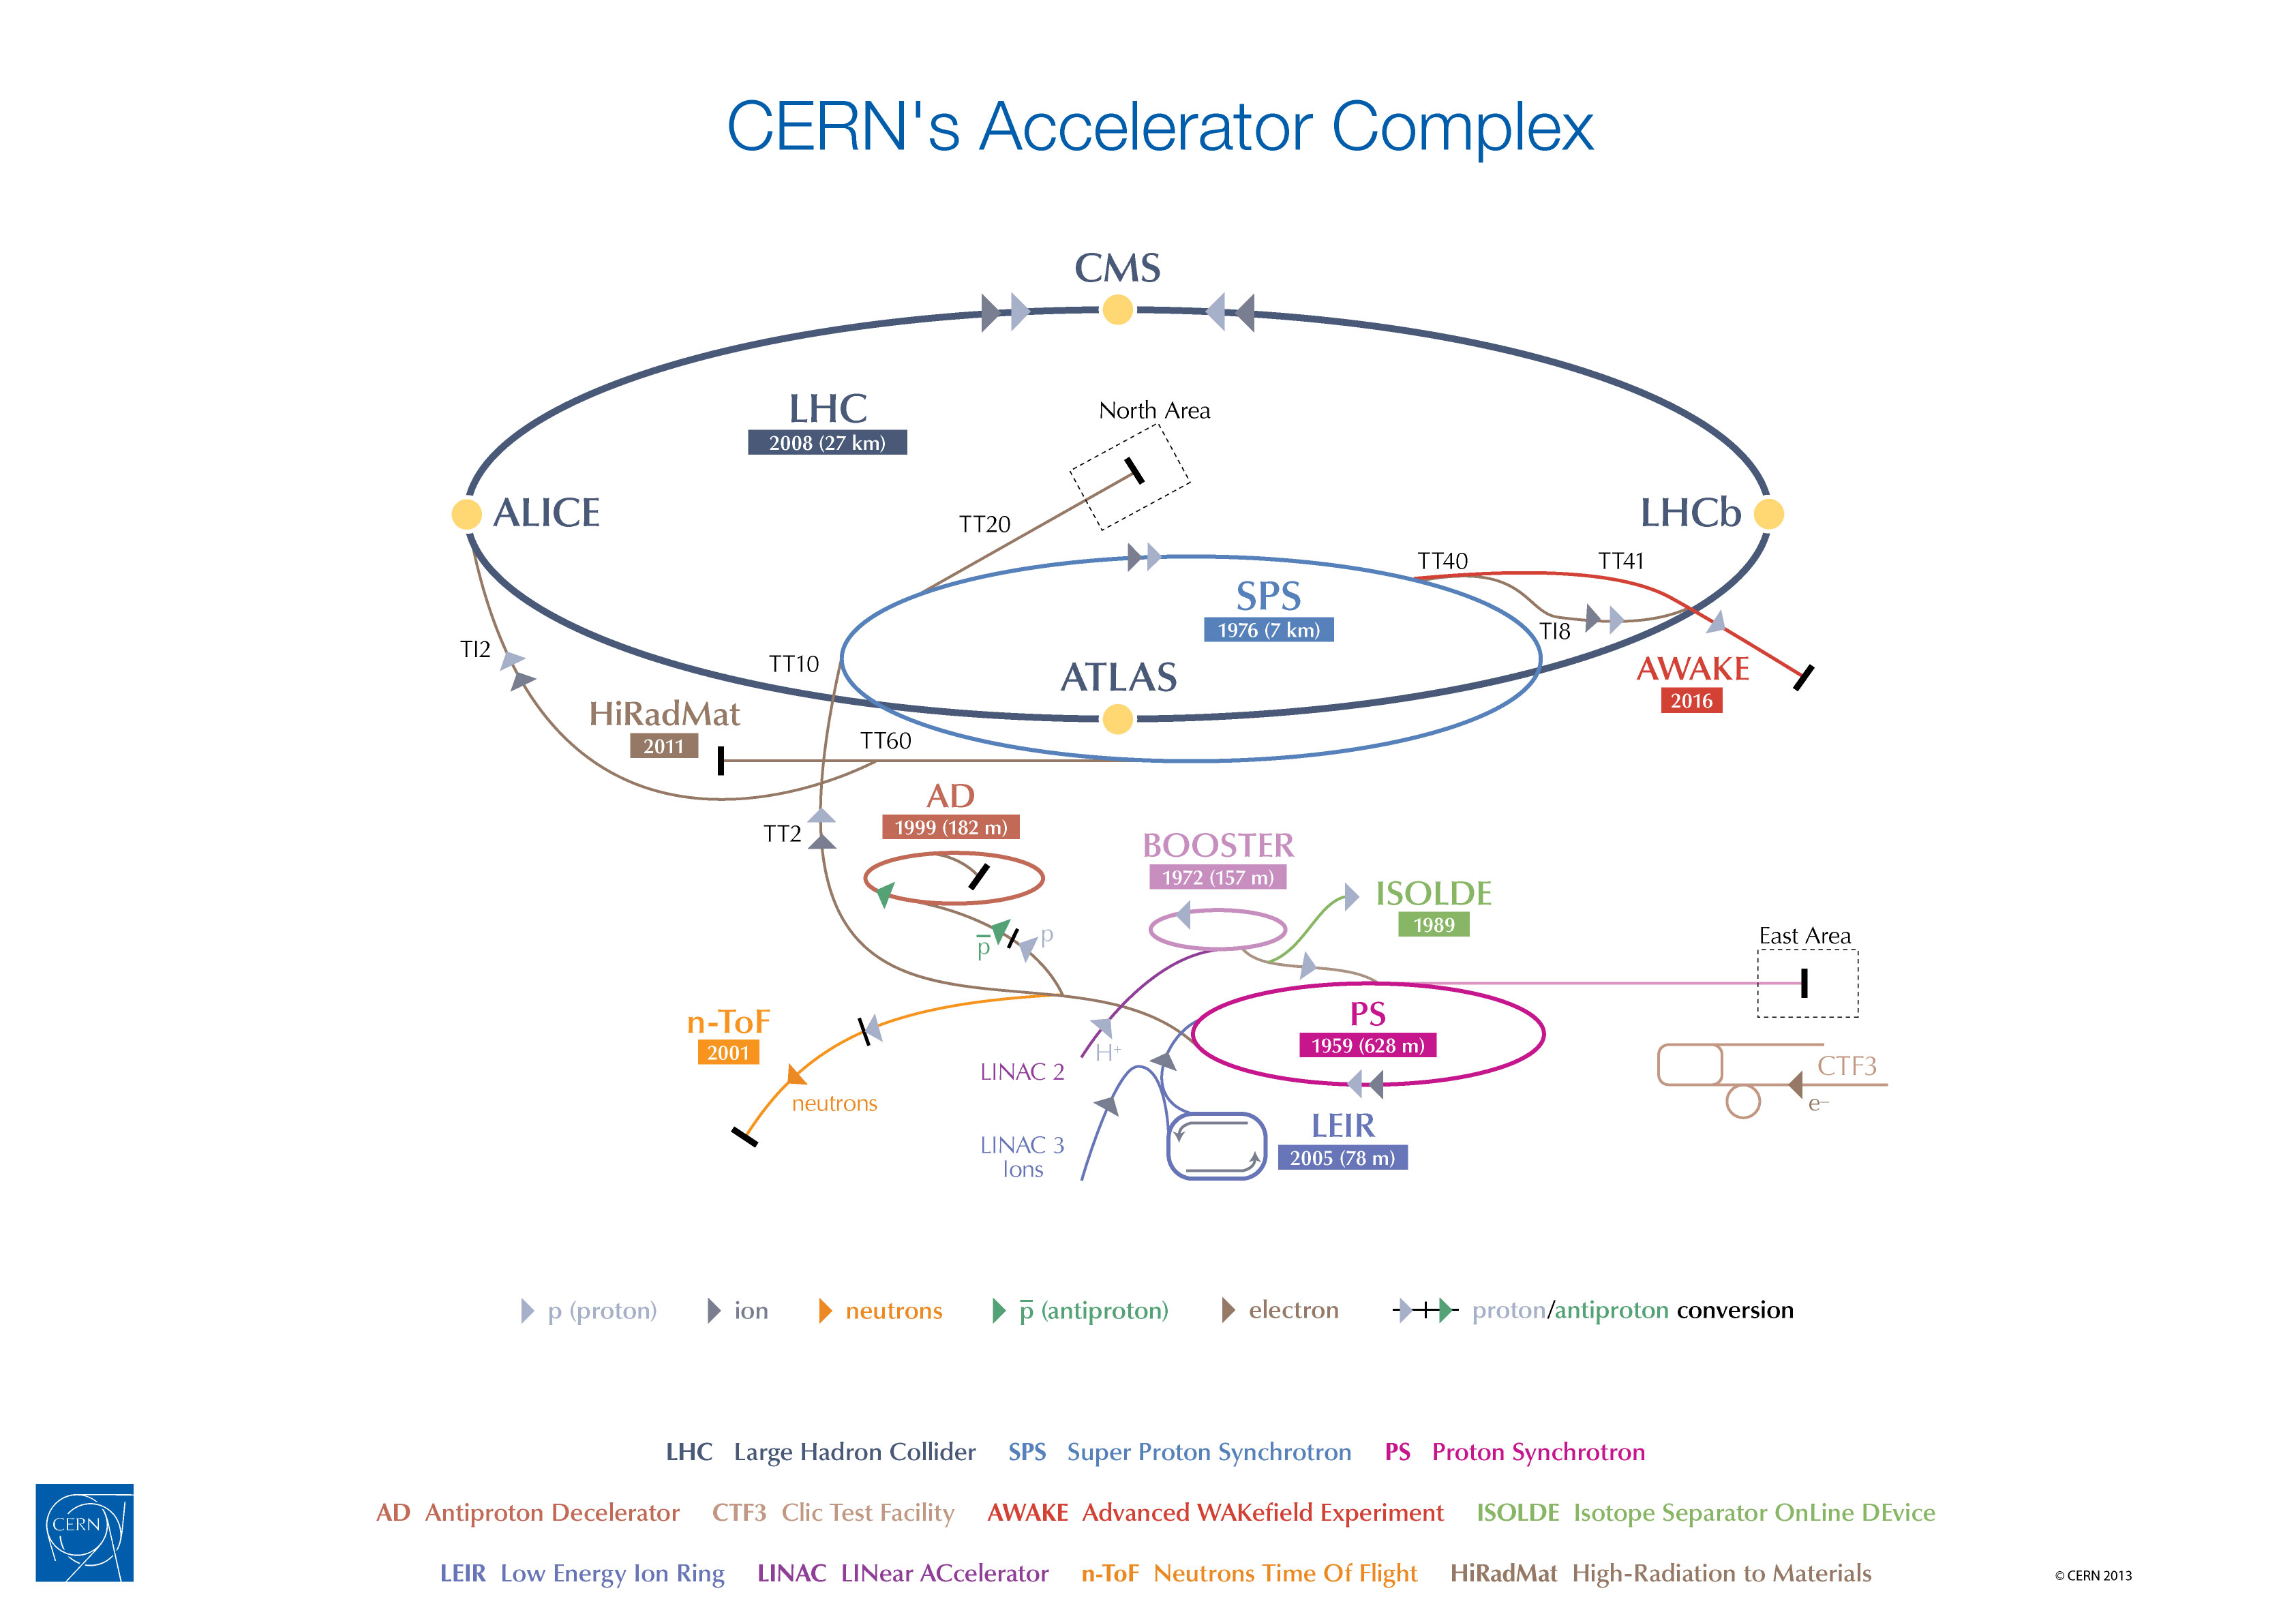
\includegraphics[width=\textwidth,clip=true,trim=10cm 0 13cm 9cm]
  {figures/lhc/cern_accelerator_complex_cds1621583}
  \caption{The CERN accelerator complex. Protons leave the Linac 2, are passed to the Booster, the
PS and SPS, before being injected in the LHC. The four main LHC experiments, CMS, ATLAS, LHCb, and
ALICE, are also shown. Figure taken from Ref.~\cite{lhc_complex}.
  \label{fig:lhc_complex}}
\end{figure}

Once inserted, beams will circulate inside the LHC beam pipes for many hours under
normal operating conditions. During this time the two beams are made to collide in four interaction
points, each containing a separate detector: 
\begin{itemize}
  \item \textbf{CMS} is a general purpose detector with a very broad physics programme covering
Standard Model measurements, Higgs physics, searches for possible new particles, et cetera. Its
main feature is the huge solenoid magnet, operating at a magnetic field strength of 3.8\unit{T}. The
CMS detector will be explained in more detail in the next chapter. 
  \item \textbf{ATLAS} is a general purpose detector like CMS, with a very similar physics
programme, but utilizing different detector techniques and magnet design. At 46\meter long, 25\meter
high and 25\meter wide, the ATLAS detector is the largest volume particle detector ever
constructed, although not as heavy as the CMS detector. 
  \item \textbf{LHCb} is a more specialized experiment, aiming to unravel the mysteries of
antimatter by studying processes involving $\cPqb$ quarks. Unlike the cylindrical CMS and ATLAS
detectors, the LHCb detector is asymmetric and targets detection of forward particles in particular.
  \item \textbf{ALICE} is a heavy-ion detector with as primary goal the study of the quark-gluon
plasma, a state of matter occuring at extreme densities. It is the main customer of the LHC
heavy-ion (lead) collision runs.
\end{itemize}
As the two beams collide with each other, or with the remaining gas in the ultrahigh vacuum of
the beam pipe, the beam
intensity keeps dropping. At a certain point more collisions can be delivered to the experiments by
starting the full chain all over again. The beam will then be dumped, and a fresh set of proton
bunches will be inserted. 
If at any time a magnet would \textit{quench}, have an increase in temperature resulting in a loss
of the superconducting state, the beams need to be dumped as well for safety reasons.  

\begin{figure}[tbp]
  \centering
  \begin{tikzpicture}
    \node[anchor=south west, inner sep=0] (image) at (0,0)
{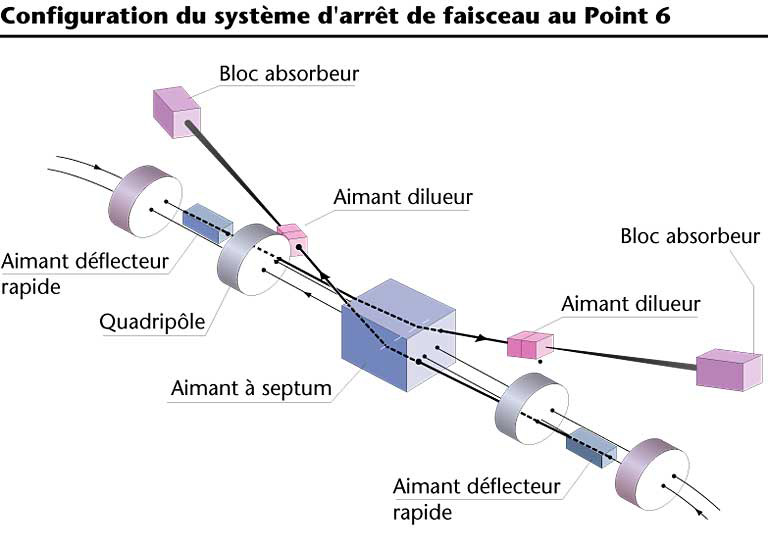
\includegraphics[width=0.8\textwidth,clip=true,trim=0 0 0 2cm]
{figures/lhc/lhc_beamdump_cds842348.jpg}};
    \begin{scope}[x={(image.south east)}, y={(image.north west)}]
      \fill[fill=white] (0.28,0.93) rectangle (0.47,1) node[pos=.5] {\small \textsf{Dump block}};
      \fill[fill=white] (0.43,0.68) rectangle (0.62,0.75) node[pos=.5] {\small \textsf{Dilutor
kicker magnet}};
      \fill[fill=white] (0.8,0.61) rectangle (1,0.67) node[pos=.5] {\small \textsf{Dump block}};
      \fill[fill=white] (0.72,0.465) rectangle (0.93,0.53) node[pos=.45] {\small \textsf{Dilutor
kicker magnet}};
      \fill[fill=white] (0.5,0.05) rectangle (0.74,0.16) node[pos=.45] {\small \textsf{Fast kicker
magnet}};
      \fill[fill=white] (0,0.5) rectangle (0.22,0.62) node[pos=.38] {\small \textsf{Fast kicker
magnet}};
      \fill[fill=white] (0.12,0.42) rectangle (0.28,0.49) node[pos=.45] {\small
\textsf{Quadrupole}};
      \fill[fill=white] (0.22,0.29) rectangle (0.44,0.36) node[pos=.45] {\small \textsf{Septum
magnet}};
     \end{scope}
  \end{tikzpicture}
  \caption{The LHC beam dump system. Figure adapted from Ref.~\cite{lhc_beamdump}.
  \label{fig:lhc_beam_dump}}
\end{figure}

The beam dump system~\cite{Schmidt:2006mi} is shown schematically in Fig.~\ref{fig:lhc_beam_dump}. 
Once the decision to dump the beam is made, a fast kicker magnet is turned on to deflect the beam
in the horizontal plane. 
This kicker magnet has a pulse rise-time of 3\mus. To accommodate this rise-time, and allow for
the safe extraction of the beam, the LHC beam structure is designed to have a gap, where there are
no filled bunches.
The kicker magnets guide the beam onto so-called septum magnets which fully extract the beam from
the beam pipe, deflecting it vertically, and steer it toward the graphite beam dump blocks. The
beam passes through a set of dilutor kicker magnets which spread the beam in both horizontal and
vertical direction, tracing out an `e' shaped path. 
The beam size increases from $0.2\mm$ to $1.5\mm$ upon reaching the dump blocks $700\meter$ away.
Without this dilution, the local beam intensity and heat production would be too large for the
blocks to handle, they would vaporize immediately. However, the graphite core of the dump block
still needs to endure temperatures of up to $750\de$C. The core has a cylindrical shape, 0.7\meter
in diameter and 7.7\meter long, and is surrounded by about 900 tons of radiation shielding blocks.


\section{Past and future running periods}

The first proton beams circled the LHC in September 2008. Unfortunately, an incident happened
shortly after, during powering tests of the dipole magnet. A faulty connection caused  an electrical
arc which punctured the helium enclosure, leading to release of helium into the insulation vacuum of
the cryostat. The pressure from the expanding helium rose too fast for the relief valves to cope,
thereby damaging dozens of magnets. It took more than one year to repair all the damage, and
install extra safety systems. 

In November 2009 beams were back in the LHC, with first stable beams
at 7\TeV centre-of-mass energy in March 2010. The LHC continued to run very smoothly throughout
2011, delivering data corresponding to an integrated luminosity of 5\fbinv to the experiments.  
In 2012 the beam energy was increased from 3.5 to 4\TeV, and also the luminosity of the beam saw a
sharp increase. A total integrated luminosity of over 20\fbinv was delivered. 

During 2013 and 2014 the LHC was shut down for maintenance and upgrade, in order to prepare the
machine to run at 13\TeV centre-of-mass energy. During these two years, the experiments at the
interaction points were also upgraded to increase detector performance in light of the changing
conditions expected upon restart. 
First stable beams for physics collisions at 13\TeV are planned for June 2015. This will signal the
start of a very exciting time for particle physics, during which our understanding of elementary
particles and their interactions will undoubtely change. 


% TODO: decide whether to put the luminosity explanation (formulae etc)
